% Requires the language-local caption macro \GelfandCanonicalInclusionCaption.
% The label on the left remains a candidate list, not a selected reading.
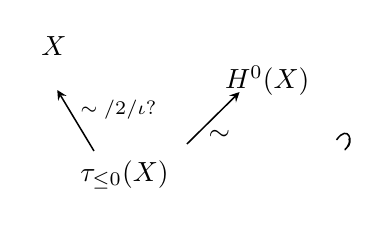
\begin{tikzpicture}[x=.88cm,y=.88cm,line width=.55pt,>=stealth]
\node at (0,1.55) {$X$};
\node at (3.08,1.05) {$H^0(X)$};
\node at (1.02,-.30) {$\tau_{\le0}(X)$};
\draw[->] (.58,.04)--(.05,.92);
\draw[->] (1.92,.14)--(2.68,.89);
\node[font=\scriptsize] at (.93,.64) {$\sim/2/\iota$?};
\node at (2.39,.26) {$\sim$};
\node[anchor=east,font=\scriptsize,align=right] at (-.10,-.33) {\GelfandCanonicalInclusionCaption};
% The isolated right-hand ink stroke has no assigned mathematical meaning.
\draw (4.08,.20) .. controls (4.25,.44) and (4.34,.16) .. (4.22,.08)
  .. controls (4.16,.02) and (4.30,.13) .. (4.26,.22);
\end{tikzpicture}
